\section{Functional analysis}
\textbf{Functional analysis of the $\beta$ and $\gamma$ functions are performed graphically together with a presentation of the restriction $\beta < -\frac{\gamma}{2}$ which has to be met in order to obtain stable structures (An $\&$ Evans 2006).} \\ 

A structure which lie in the region where $\beta > -\frac{\gamma}{2}$ might be created, but as soon as the time integration begins the structure will no longer be stable. This unstable region is shown in figure 19 as a pink region in the upper right corners of each subplot. It has been found to be unstable by An $\&$ Evans in 2006;i.e. for a cusped density profile which goes as $r^{\gamma}$ near the center, the limiting value of the anisotropy parameter $\beta$ cannot be greater than $-\frac{\gamma}{2}$ at the center. It follows from the non-negativity of the phase-space density. By tuning the two parameters $r_a$ (anisotropy radius) and $r_s$ (scale radius) it is possible to approach the unstable region without ever crossing into it. This knowledge is helpful when choosing how to set up the initial structure; If one wishes to create a stable structure close to or far away from the unstable region one simply has to make the corresponding choices for these two parameters. We learn from figure 19 that a small value of $r_a$, a large value of $r_s$ can bring our structure closer to the unstable region. Notice how these effects are unaffected by our choice of $\rho_0$ as it is a constant that will not affect the differentiation performed when computing the $\gamma$ array. But in practical purposes it is best to make some compromise to avoid too large of a computational cost (longer simulation time). Also, there is no guarantee that a structure outside the unstable region is stable. This has to be checked. In fact the contrary might be true as well; It might be possible to create a stable structure that crosses into the pink region and out again, since the An $\&$ Evans paper from 2006 only concludes this instability based on a smooth $\gamma$-profile. 
\begin{figure}[!htbp]
\centering
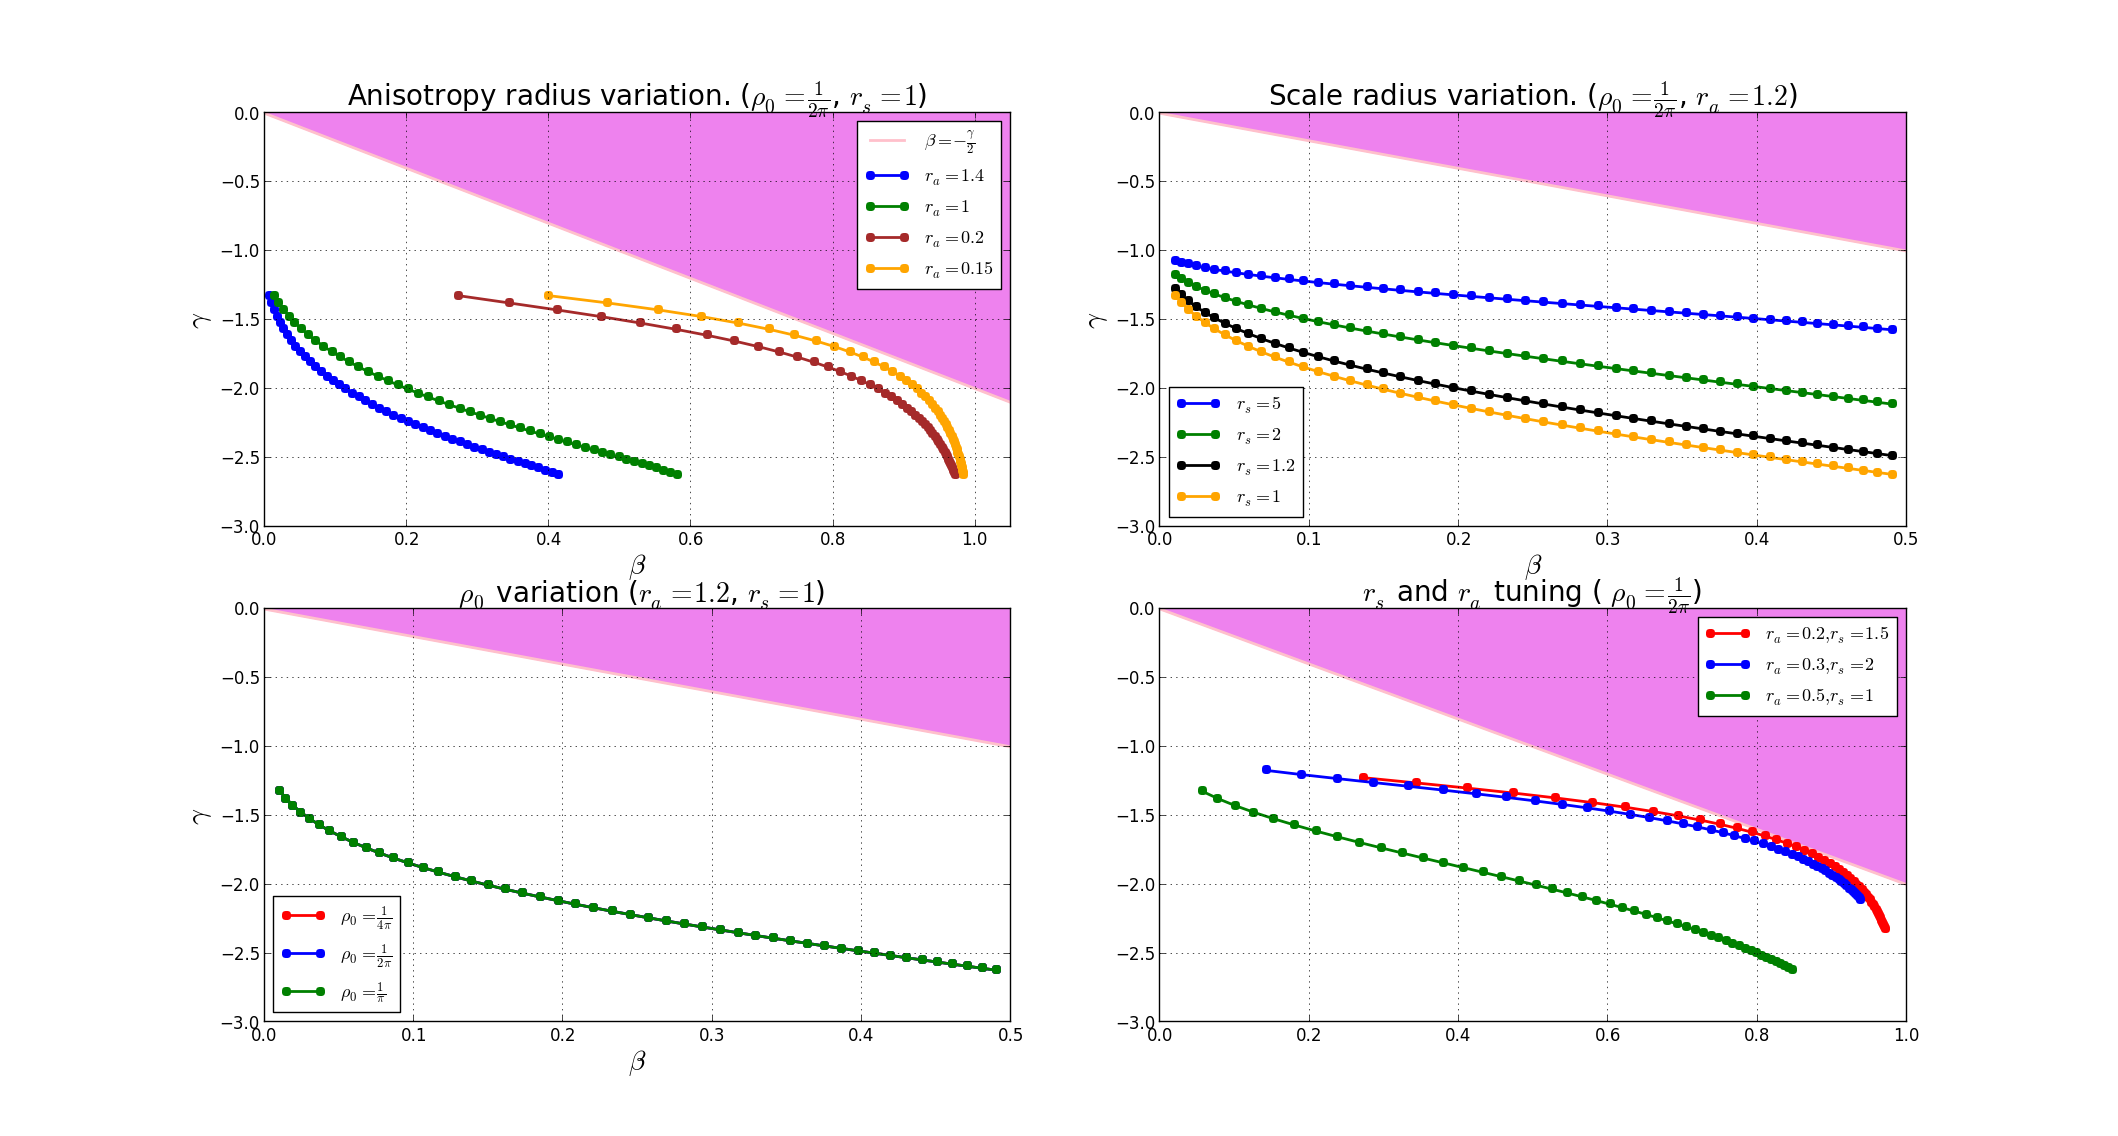
\includegraphics[width=1.0\linewidth]{img/beta_gamma_functions.png}
\caption{Analysis of the $\beta$ and $\gamma$ functional expressions for different choices of scale radius and anisotropy radius. The $\rho_0$ normalization parameter is kept fixed at $\rho_0 = \frac{1}{2 \pi}$. Plotted together with the unstable region where $\beta > -\frac{\gamma}{2}$. This figure gives a qualititive idea of the kind of structures that might fall into the stable category.}
\label{fig:test}
\end{figure}
\begin{figure}[!htbp]
\centering
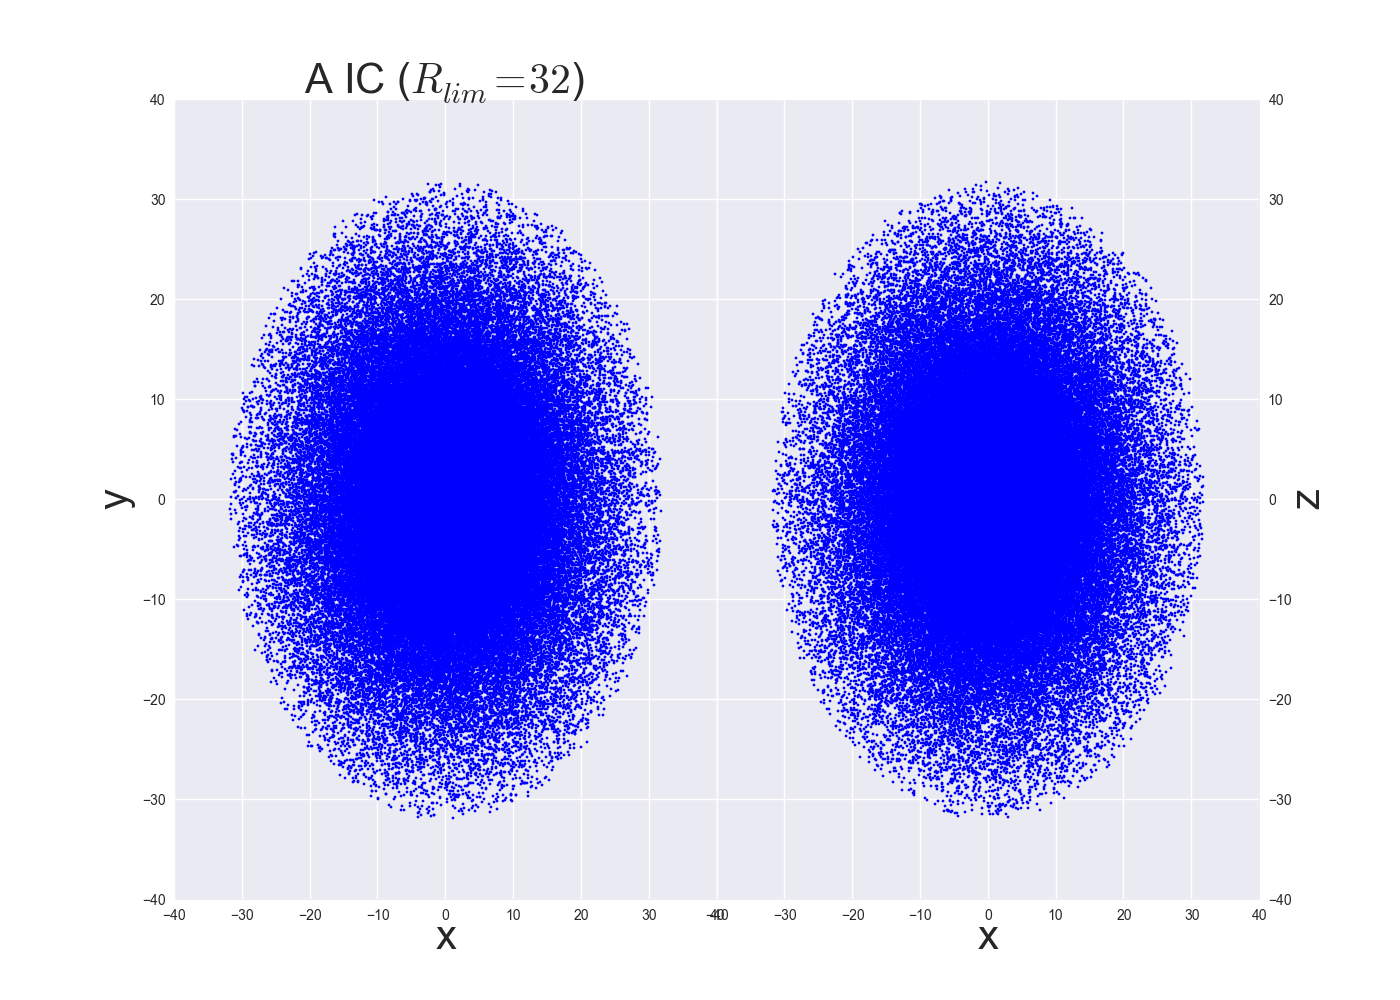
\includegraphics[width=1.0\linewidth]{img/A_IC_xy_xz.png}
\caption{2D view of IC for structure A. we first see the particles y-positions vs. their x-positions and then their z-positions vs. their x-positions. The halo is cut off at a radius of $R_{lim}=32$.}
\label{fig:test}
\end{figure}
For all structures, the characteristic radius is $r_s = 1$, and the normalization constant $\rho_0 $ has been chosen so that the total mass inside $r = 13r_s$ is 1. This ensures that the dynamical time mentioned in the previous section , for particles inside $r = 13r_s$ is smaller than 100 time units (which is the duration of all simulations performed). For the Osipkov-Merritt model, we have seen in the previous section that the $\beta$ profile is 
\begin{equation}
\beta = \frac{r^2}{r^2 + r_a^2}  
\end{equation}
The anisotropy radius $r_a$ is varied from $1.2 r_s$ to $ 0.2 r_s $. When $r_a$ exceeds $r_s$ instabilities can be avoided. It is shown (Kazantzidis, Stelios)  that $r_a \geq 1.33r_s$ will ensure stability. In the setup the particle number is varied from $ 10^4 $ to $ 10^6 $.